\documentclass{article}

\usepackage{amsmath, amsthm, amssymb, amsfonts}
\usepackage{thmtools}
\usepackage{graphicx}
\usepackage{setspace}
\usepackage{geometry}
\usepackage{float}
\usepackage{hyperref}
\usepackage[utf8]{inputenc}
\usepackage[english]{babel}
\usepackage{framed}
\usepackage[dvipsnames]{xcolor}
\usepackage{tcolorbox}
\usepackage{physics}
\DeclareMathOperator{\grd}{grad}
\colorlet{LightGray}{White!90!Periwinkle}
\colorlet{LightOrange}{Orange!15}
\colorlet{LightGreen}{Green!15}

\newcommand{\HRule}[1]{\rule{\linewidth}{#1}}

\declaretheoremstyle[name=Theorem,]{thmsty}
\declaretheorem[style=thmsty,numberwithin=section]{theorem}
%\tcolorboxenvironment{theorem}{colback=LightGray}

\declaretheoremstyle[name=Proposition,]{prosty}
\declaretheorem[style=prosty,numberlike=theorem]{proposition}
\tcolorboxenvironment{proposition}{colback=LightOrange}

\declaretheoremstyle[name=Principle,]{prcpsty}
\declaretheorem[style=prcpsty,numberlike=theorem]{principle}
\tcolorboxenvironment{principle}{colback=LightGreen}

\setstretch{1.2}
\geometry{
    textheight=9in,
    textwidth=5.5in,
    top=1in,
    headheight=12pt,
    headsep=25pt,
    footskip=30pt
}

% ------------------------------------------------------------------------------

\begin{document}

% ------------------------------------------------------------------------------

\section*{Curve Integrals}

Recall (or accept) from physics that the work 
(which has the same units as energy) done by a constant force $F$ over a distance $D$ is 
$W=FD$. This describes the case of the force pointing in the direction
of motion. A slightly more general equation is $W = F \cdot D$, where
$F$ is the force vector and $D$ is the displacement vector (imagine pushing a box). But this 
equation still assumes a straight-line displacement and constant force in a fixed direction.
What if our trajectory is a curve $C(t)$ and the force is a vector quantity $F(X)$ that depends
on position?

If one zooms in close enough on a continuous vector field, it looks
constant, and similarly a curve will look like a straight line segment.
The work done by the force on a small time interval $(t, t + \Delta t)$ can then be approximated as 
\[F(C(t))\cdot (C(t+\Delta t)-C(t)).\]
We can rewrite this as 
\[F(C(t))\cdot \frac{C(t+\Delta t) - C(t)}{\Delta t}\Delta t.\]
If we add up these small bits of work and let $\Delta t \to 0$, we end
up with an integral.

Thus we define the \textbf{integral of $F$ along $C$} from time $a$ to time $b$ as 
\[\int_C F = \int_a^b F(C(t))\cdot \frac{dC}{dt} dt.\]

\textbf{Example.} $F(x,y) = (x^2y, y^3)$. Find the integral along the straight line
from $(0,0)$ to $(1,1)$.

We take $C(t) = (t,t)$, $0 \leq t \leq 1$. $C'(t) = (1,1)$. Then 
\[F(C(t)) = (t^3,t^3).\]
Our integral is then
\[\int_0^1 (t^3,t^3)\cdot (1,1)dt = \int_0^1 2t^3 dt = 1/2.\]

In $2$-space, if we write $F = (f,g)$, $C(t) = (x(t),y(t))$, then the curve integral
can be expressed
\[\int_C F = \int_C fdx + gdy.\]
Symbolically, the expression $fdx + gdy = (f,g)\cdot (dx,dy)$. So one can write
\[\int_C F = \int_a^b \left[ f(x(t),y(t))\frac{dx}{dt} + g(x(t),y(t))\frac{dy}{dt}\right]dt.\]

\textbf{Remark:} The curve integral is independent of the particular 
parametrization you take. That is, if $C_1(t)$ and $C_2(t)$ trace out the same
curve but proceed at different rates, the integral of $F$ over either
curve will be the same.

\textbf{Example.} Compute the integral of $F(x,y) = (x^2, xy)$ on the parabola $x=y^2$ from $(1,-1)$ to $(1,1)$.

We can parametrize our curve as $C(t) = (t^2, t)$, $-1 \leq t \leq 1$. The integral is then
\[\int_C F \cdot dC = \int_{-1}^1 f(C(t))\cdot C'(t)dt = \int_{-1}^1(t^4,t^3)\cdot(2t+1)dt = \int_{-1}^1 (2t^5 + t^3)dt.\]

\textbf{Example.} Let 
\[G(x,y) = \left( \frac{-y}{x^2+y^2}, \frac{x}{x^2+y^2} \right).\]
Integrate $G$ on the circle of radius $3$ centered at the origin from $(3,0)$ to $(3\sqrt{3}/2, 3/2)$.

We can parametrize the curve $C$ as $C(t) = (3\cos t, 3\sin t)$ where $0 \leq t \leq \pi/6$, so that 
$C'(t) = 3(-\sin t, \cos t)$. Now,
\[G(C(t)) = \left(\frac{-3\sin t}{9}, \frac{3\cos t}{9}\right) = \frac{1}{3}(-\sin t, \cos t).\]
So the curve integral is 
\[\int_0^{\pi/6} G(C(t))\cdot C'(t)dt = \int_0^{\pi/6} \frac{1}{3}(-\sin t,\cos t)\cdot [3(-\sin t,\cos t)]dt=\pi/6.\]
Notice that $\pi/6$ is also the change in angle of the parametrized particle over the course of its journey. 
This is not a coincidence.

\section*{An Aside on Differential Forms}
A function $f(x,y,z)$ has gradient
\[\grd f = \left( \frac{\partial f}{\partial x}, \frac{\partial f}{\partial y}, \frac{\partial f}{\partial z} \right).\]
The \textbf{total differential} of $f$ is 
\[df = \frac{\partial f}{\partial x} dx + \frac{\partial f}{\partial y} dy + \frac{\partial f}{\partial z}dz.\]
You can view this as a purely symbolic thing, perhaps a fancier way of writing the gradient. However, there is something
meaningful about this expression. If we think of $dx,dy,dz$ as small changes in $x$, $y$, and $z$, then 
this expression gives a way of approximating the corresponding change in $f$. Remember that differentiability means that 
for $H$ in some small enough neighborhood of the origin, we can write
\[f(X+H) - f(X) = \grd f(X) \cdot H + \norm{H} g(H)\]
where $g(H) \to 0$ as $H \to 0$. The left hand side is the change in $f$, say $\Delta f$, going from $X$ to $X+H$.
$H$ itself is the change in input, which we could write $H = (\Delta x, \Delta y, \Delta z)$, where we 
imagine these are small changes in $x$, $y$, and $z$. Dropping the ``error'' term $\norm{H}g(H)$, this reads
\[\Delta f \approx \frac{\partial f}{\partial x} \Delta x + \frac{\partial f}{\partial y} \Delta y + \frac{\partial f}{\partial z} \Delta z. \]

\section*{Back to Curve Integrals}
Given $x = r\cos\theta$ and $y = r\sin\theta$, we can form their total differentials
\[dx = \cos\theta dr - r \sin\theta d\theta,\ dy = \sin\theta dr + r\cos\theta d\theta.\]
This is equivalent to 
\[dx = \cos\theta dr - yd\theta,\ dy = \sin\theta dr + x d\theta.\]
We can rewrite this as 
\[dx = \frac{x}{\sqrt{x^2+y^2}}dr - yd\theta,\ dy = \frac{y}{\sqrt{x^2+y^2}}dr + x d\theta.\]
In turn, we can say
\[-ydx = \frac{-xy}{\sqrt{x^2+y^2}}dr - y^2d\theta,\ dy = \frac{xy}{\sqrt{x^2+y^2}}dr + x^2 d\theta.\]
Finally, adding these two equations together and solving for $d\theta$ yields,
\[d\theta = \frac{-y}{x^2+y^2}dx + \frac{x}{x^2+y^2}dy. \]
This differential form is telling us that integral of the right hand side above will \emph{always give the change in angle
of the position vector over the course of traversing the curve.}

A \textbf{path} $C$ is a sequence of curves $C_1, \ldots, C_m$ where each $C_i$ is defined on an interval
$[a_i,b_i]$ and if we write $P_i = C_i(a_i)$ and $Q_i = C_i(b_i)$, then $P_{i+1}=Q_i$. In other words, one curve
ends where the next one starts. The integral along such a path $C$ is defined as 
\[\int_C F := \int_{C_1} F + \cdots + \int_{C_m} F.\]

A \textbf{closed path} is one such that $Q_m = P_1$ (we close the loop).

\textbf{Example.} Evaluate the integral of $F = (x^2,xy)$ along the closed path that goes along $y=x^2$ from
$(0,0)$ to $(1,1)$, then along the line $y=x$ from $(1,1)$ back to $(0,0)$. 

We can parametrize this path as two curves $C_1$ and $C_2$. Where $C_1(t) = (t,t^2)$, $0 \leq t \leq 1$
and $C_2(t) = (1-t, 1-t)$, $0 \leq t \leq 1$. The integral then becomes
\[\int_C F = \int_{0}^1 (t^2, t^3)\cdot(1, 2t)dt + \int_0^1 ((1-t)^2, (1-t)^2)\cdot(-1,-1)dt = -\frac{1}{3} + \frac{2}{5}.\]

\section*{The Reverse Path}

For a curve $C$ defined for $a\leq t \leq b$, the \textbf{reverse curve} $C^-$ is defined by 
\[C^- = C(a+b-t), a \leq t \leq b.\]

\textbf{Lemma.} As one might expect, we have 
\[\int_{C^-} F = - \int_C F. \]
This comes from using $u = a + b - t$, $du = -dt$.

\textbf{Example.} Integrate $F(x,y) = (x^2,xy)$ along $y=x$
from $(1,1)$ to $(0,0)$. We can use the lemma and instead integrate 
along the reverse curve and flip the sign of the result. So let $C(t) = (t,t)$, 
$0 \leq t \leq 1$. Then what we're after is 
\[-\int_0^1 2t^2 dt = -2/3.\]

The \textbf{reverse path} of $C_1, \ldots, C_m$ is 
$C_m^-, \ldots, C_1^-$.

\section*{Path Integrals and Potentials}

\textbf{Theorem.} Let $F$ be a vector field on an open set $U$ and
suppose $F = \grd \varphi$ for some $\varphi$ on $U$. Let $C$
be a path from $P$ to $Q$. Then 
\[\int_C F = \varphi(Q) - \varphi(P).\]
In particular, there is no dependence on the path itself, only
on the endpoints.
\begin{proof}
    Let $g(t) = \varphi(C(t))$. Then $g'(t) = \grd \varphi(C(t))\cdot C'(t)$.
    Then we have
    \[\int_C F = \int_a^b F(C(t))\cdot C'(t)dt = \int_a^b \grd \varphi(C(t))\cdot C'(t)dt.\]
    This last integral is the integral of $g'(t)$ from $a$ to $b$, so this becomes 
    \[\int_C F = \int_a^b g'(t) dt = g(t) \bigg\vert_a^b = \varphi(C(b)) - \varphi(C(b)) = \varphi(Q) - \varphi(P).\]
\end{proof}

\textbf{Corollary.} The integral around any closed loop of a conservative vector
field is $0$. This is because such an integral will end up evaluating to $\varphi(P) - \varphi(P) = 0$.

Notice this gives a test: if you can find a closed loop $C$ with $\int_C F \neq 0$,
then $F$ is certainly not conservative.


\textbf{Example.} Let \[F(x,y,z) = (2xy^3z, 3x^2y^2z, x^2y^3).\]
Then 
\[\varphi(x,y,z) = x^2y^3z\]
is a potential. Let $P=(1,-1,2)$ and $Q=(-3,2,5)$. Then for any path 
from $P$ to $Q$, we have \[\int_P^Q F = \varphi(Q) - \varphi(P) = 360 - (-2) = 362.\]
When working with a conservative vector field, the notation $\int_P^Q$ is fine 
since there's no dependence on the particular path.

\textbf{Example}. Integrating
\[G(x,y) = \left( \frac{-y}{x^2+y^2}, \frac{x}{x^2+y^2}\right)\]
around the unit circle yields a nonzero value, which shows
$G$ is not conservative. The computation will be a homework problem.

\textbf{Example.} Let $G(x,y)$ be as above. Compute the integral along 
the straight segment path going from $(0,0)$ to $(1,1)$ to $(0,1)$.

\section*{Dependence of the Integral on the Path}

\textbf{Theorem.} Let $U$ be a connected open set and let $F$ be a
vector field on $U$. Assume that for any two points $P,Q \in U$ the integral
\[\int_{P,C}^Q F\]
is independent of the path $C$ in $U$ joining $P$ and $Q$. There there exists
a potential function for $F$ on $U$.
\begin{proof}
    Fix some point $P_0 \in U$, then define
    \[\varphi(X) = \int_{P_0}^X F.\]
    Write $F = (f_1, \ldots, f_n)$. We must investigate the quantity
\[\frac{\varphi(X + h E_i) - \varphi(X)}{h} = \frac{1}{h} \left[ \int_{P_0}^{X+hE_i} F - \int_{P_0}^X F \right].\]
We aim to show that this tends to $f_i$ as $h \to 0$.
By path independence, we can split the first integral as 
$\int_{P_0}^X + \int_X^{P_0 + hE_i}$, which gives us
\[\frac{\varphi(X + h E_i) - \varphi(X)}{h} = \frac{1}{h} \left[ \int_{X}^{X+hE_i} F  \right].\]
We can compute this integral by taking the path 
\[C(t) = X + thE_i,\ 0 \leq t \leq 1.\]
$C'(t) = hE_i$, and $F(C(t)) = F(X + thE_i)$. Notice that $F \cdot E_i = f_i$. The path integral becomes
\[\frac{\varphi(X + h E_i) - \varphi(X)}{h} = \frac{1}{h}\int_0^1 f_i(X+thE_i)hdt.\]
If we change variables as $u=th$, $du = hdt$, we obtain
\[\frac{\varphi(X + h E_i) - \varphi(X)}{h} = \frac{1}{h}\int_0^h f_i(X+uE_i)du.\]
Letting $h \to 0$, the fundamental theorem of calculus tells us the right
side tends to $f_i(X)$. 
\end{proof}

\textbf{Theorem.} Let $U$ be an open connected set, and let $F$ be 
a vector field on $U$. If the integral of $F$ around every closed path
in $U$ is $0$, then $F$ has a potential.
\begin{proof}
    Let $P,Q$ be points in $U$, and let $C$ and $D$ be paths from $P$ to $Q$ in $U$.
    Then $C$ followed by $D^-$ is a closed loop, so that 
    \[\int_C F + \int_{D^-} F = 0,\]
    which implies
    \[\int_C F = \int_D F.\]
    Now we apply the previous theorem.
\end{proof}

We now have a pretty remarkable theorem.

\textbf{Theorem.} Let $F$ be a vector field defined on the plane minus the origin.
Write $F = (f,g)$. Assume $D_2 f = D_1 g$. Let $C$ be the counterclockwise unit circle
centered at the origin. If $\int_C F = 0$, then $F$ has a potential. Otherwise,
writing \[k = \frac{1}{2\pi} \int_C F,\]
the field \[F - kG\] has a potential, where $G$ is our special example.
\begin{proof}
    First suppose $\int_C F = 0$. For $X \neq 0$, define $\varphi(X)$ to be 
    the integral along the path in the figure.
    \begin{figure}[h]
        \centering
        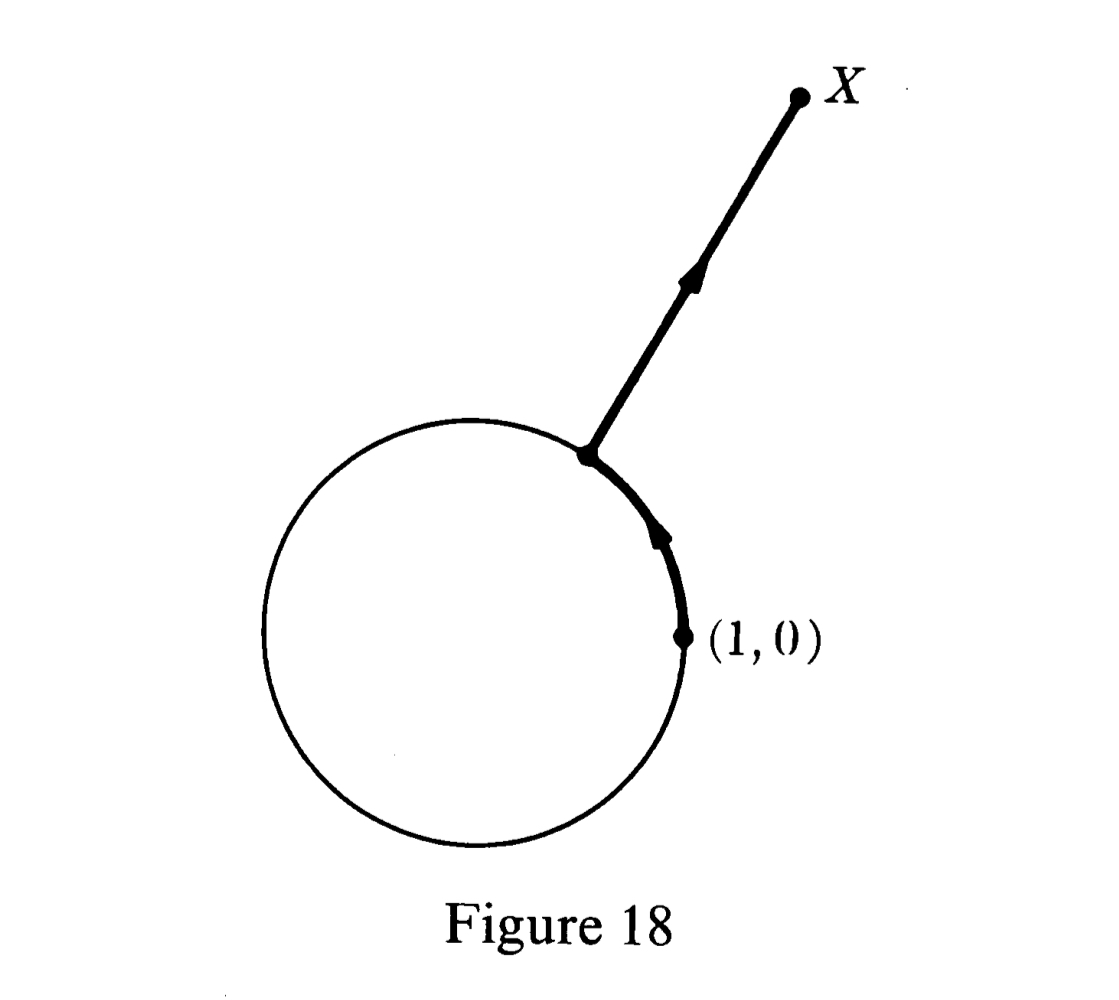
\includegraphics[scale = 0.15]{contour.jpeg}
    \end{figure}
    That is, we get to $X$ by first walking along the circle until we 
    are standing at the correct angle, and then proceed radially outward/inward to the point $X$.
    Our assumption ensures that $\varphi$ is well-defined. Similar techniques to the previous
    theorems will show that $\grd \varphi = F$.

    In the second case, $F-kG$ has $0$ integral around $C$, so then the first
    case applies.
\end{proof}

\end{document}
